\documentclass[11pt]{beamer}
% \usetheme{Boadilla}
  \usetheme{default}


% acronyms for text or math mode
\newcommand {\ccast} {\mbox{\small CCAST}}
\newcommand {\cris} {\mbox{\small CrIS}}

\newcommand {\airs} {\mbox{\small AIRS}}
\newcommand {\iasi} {\mbox{\small IASI}}
\newcommand {\idps} {\mbox{\small IDPS}}
\newcommand {\nasa} {\mbox{\small NASA}}
\newcommand {\noaa} {\mbox{\small NOAA}}
\newcommand {\nstar} {\mbox{\small STAR}}
\newcommand {\umbc} {\mbox{\small UMBC}}
\newcommand {\uw}   {\mbox{\small UW}}

\newcommand {\fft}  {\mbox{\small FFT}}
\newcommand {\ifft} {\mbox{\small IFFT}}
\newcommand {\fir}  {\mbox{\small FIR}}
\newcommand {\fov}  {\mbox{\small FOV}}
\newcommand {\for}  {\mbox{\small FOR}}
\newcommand {\ict}  {\mbox{\small ICT}}
\newcommand {\ils}  {\mbox{\small ILS}}
\newcommand {\igm}  {\mbox{\small IGM}}
\newcommand {\opd}  {\mbox{\small OPD}}
\newcommand {\rms}  {\mbox{\small RMS}}
\newcommand {\zpd}  {\mbox{\small ZPD}}
\newcommand {\ppm}  {\mbox{\small PPM}}
\newcommand {\srf}  {\mbox{\small SRF}}

\newcommand {\ES} {\mbox{\small ES}}
\newcommand {\SP} {\mbox{\small SP}}
\newcommand {\IT} {\mbox{\small IT}}
\newcommand {\SA} {\mbox{\small SA}}

\newcommand {\ET} {\mbox{\small ET}}
\newcommand {\FT} {\mbox{\small FT}}

% abbreviations, mainly for math mode
\newcommand {\real} {\mbox{real}}
\newcommand {\imag} {\mbox{imag}}
\newcommand {\atan} {\mbox{atan}}
\newcommand {\obs}  {\mbox{obs}}
\newcommand {\calc} {\mbox{calc}}
\newcommand {\sinc} {\mbox{sinc}}
\newcommand {\psinc} {\mbox{psinc}}
\newcommand {\std} {\mbox{std}}

% symbols, for math mode only
\newcommand {\wnum} {\mbox{cm$^{-1}$}}
\newcommand {\lmax} {L_{\mbox{\tiny max}}}
\newcommand {\vmax} {V_{\mbox{\tiny max}}}

\newcommand {\tauobs} {\tau_{\mbox{\tiny obs}}}
\newcommand {\taucal} {\tau_{\mbox{\tiny calc}}}
\newcommand {\Vdc}  {V_{\mbox{\tiny DC}}}

\newcommand {\rIT} {r_{\mbox{\tiny\textsc{ict}}}}
\newcommand {\rES} {r_{\mbox{\tiny\textsc{es}}}}
\newcommand {\robs} {r_{\mbox{\tiny obs}}}

\newcommand {\rITobs} {r_{\mbox{\tiny\textsc{ict}}}^{\mbox{\tiny obs}}}
\newcommand {\rITcal} {r_{\mbox{\tiny\textsc{ict}}}^{\mbox{\tiny cal}}}

\newcommand {\ITmean} {\langle\mbox{\small IT}\rangle}
\newcommand {\SPmean} {\langle\mbox{\small SP}\rangle}


\title{ccast intro and overview}
\author{H.~E.~Motteler}
\institute{
  UMBC Atmospheric Spectroscopy Lab \\
  Joint Center for Earth Systems Technology \\
}
\date{\today}
\begin{document}

%----------- slide --------------------------------------------------%
\begin{frame}[plain]
\titlepage
\end{frame}
%----------- slide --------------------------------------------------%
\begin{frame}
\frametitle{introduction}

\ccast\ takes level zero data from the Cross-track Infrared Sounder
(CrIS), a Fourier transform spectrometer on the Suomi NPP and JPSS
weather satellites, and produce high-quality calibrated radiances.
It is written primarily in Matlab, allowing for easy interaction,
modification, and data visualization.  We give a brief overview of
the design, implementation, and use.

\hspace{2cm}

The authors of the \umbc\ \ccast\ are Howard E.~Motteler, David Tobin,
L.~Larrabee Strow, and Dan Mooney, with interferometric parameters
in spreadsheet form from Joe Predina.

\hspace{2cm}

\ccast\ is available as a GitHub public repository and is distributed
under the terms of the GNU GPL v3.

\end{frame}
%----------- slide --------------------------------------------------%
\begin{frame}
\frametitle{history}

\begin{itemize}
  \item \ccast\ started as a collaboration between \umbc\ and
    \uw\ in fall 2011, with major components from the 2007-2008 FM1
    bench and TVAC tests.

  \item H.~Motteler wrote the L1a processing, starting with Dan
    Mooney's RDR reader, and L.~Strow, Dave Tobin, and H.~Motteler
    all collaborated on the L1b 

  \item this forked into a \uw\ version with Fred Nagel's geo that
    got first light, and a \umbc\ version with \noaa\ geo that got
    the first high res obs a month later.

  \item in the summer of 2012 H.~Motteler updated the UW code to 
    run in the \umbc\ environment, and for some time maintained both
    versions while continuing to develop the \umbc\ branch.

  \item major portions of the \uw\ branch, including \ict\ modeling
    and the non-linearity correction, were updated and merged into
    the \umbc\ branch.
\end{itemize}


\end{frame}
%----------- slide --------------------------------------------------%
\begin{frame}
\frametitle{preprocessing}

\begin{center}
  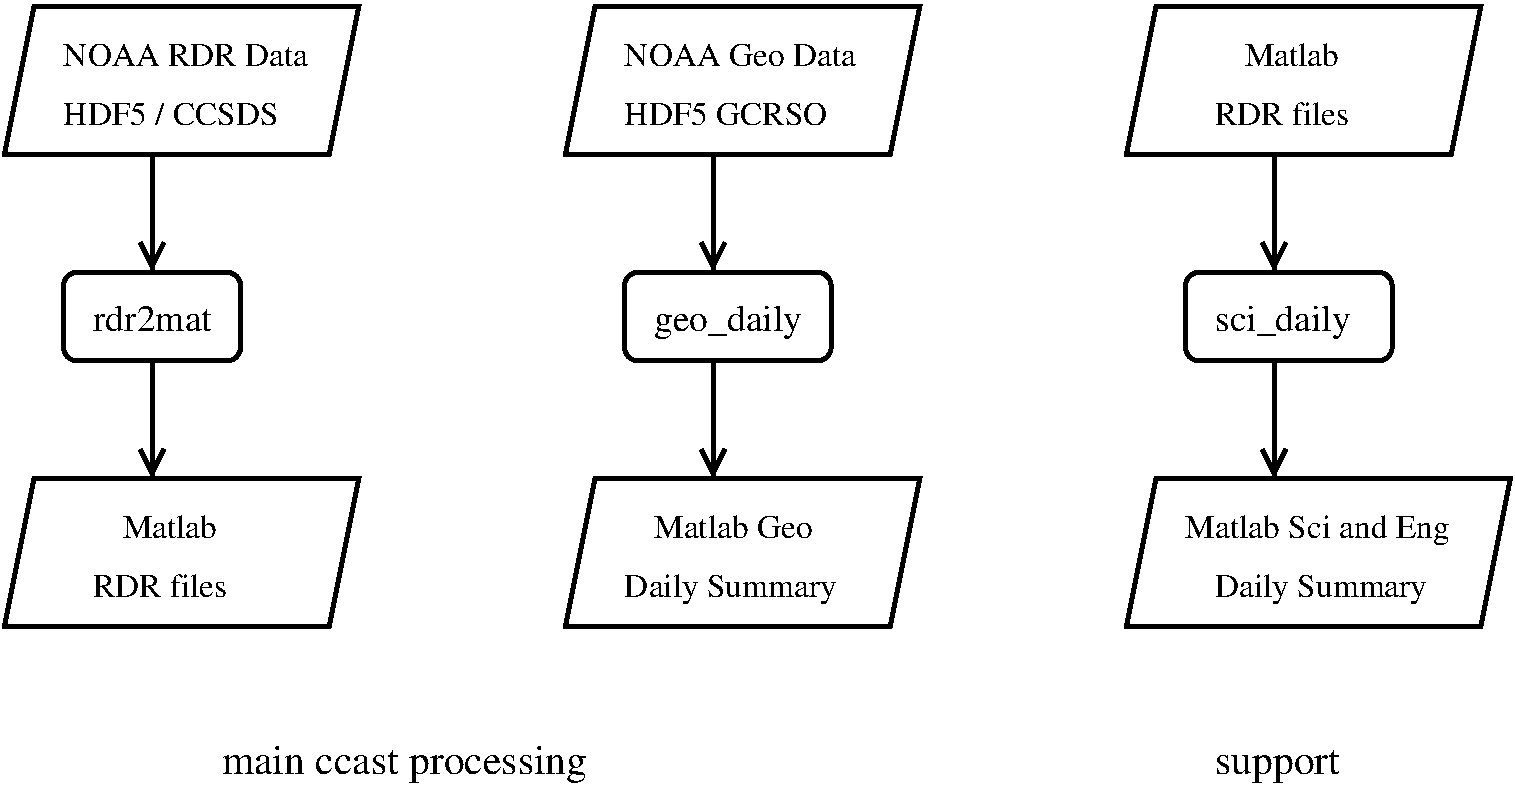
\includegraphics[scale=0.4]{figures/prepro.pdf}
\end{center}

\end{frame}
%----------- slide --------------------------------------------------%
\begin{frame}
\frametitle{preprocessing}

\ccast\ processing is done in two passes---the first pass takes HDF
and CCSDS data to Matlab RDR files, and the second takes the Matlab
RDR files to calibrated radiances.  The top-level preprocessing
script is ccast\_prepro.  The main steps there are

\begin{itemize}
  \item rdr2mat -- read \noaa\ RDR files (CCSDS level 0 data with an
    HDF-5 wrapper) and produce Matlab RDR files

  \item geo\_daily -- read \noaa\ GCRSO HDF-5 geo files and produce
    daily abstracts of CrIS geo data, as Matlab files.

  \item sci\_daily -- read Matlab RDR files and produce daily
    abstracts of ``science'' (8~second) and ``engineering''
    (4~minute) support data, as Matlab files.

\end{itemize}

\end{frame}
%----------- slide --------------------------------------------------%
\begin{frame}
\frametitle{main processing}

\begin{center}
  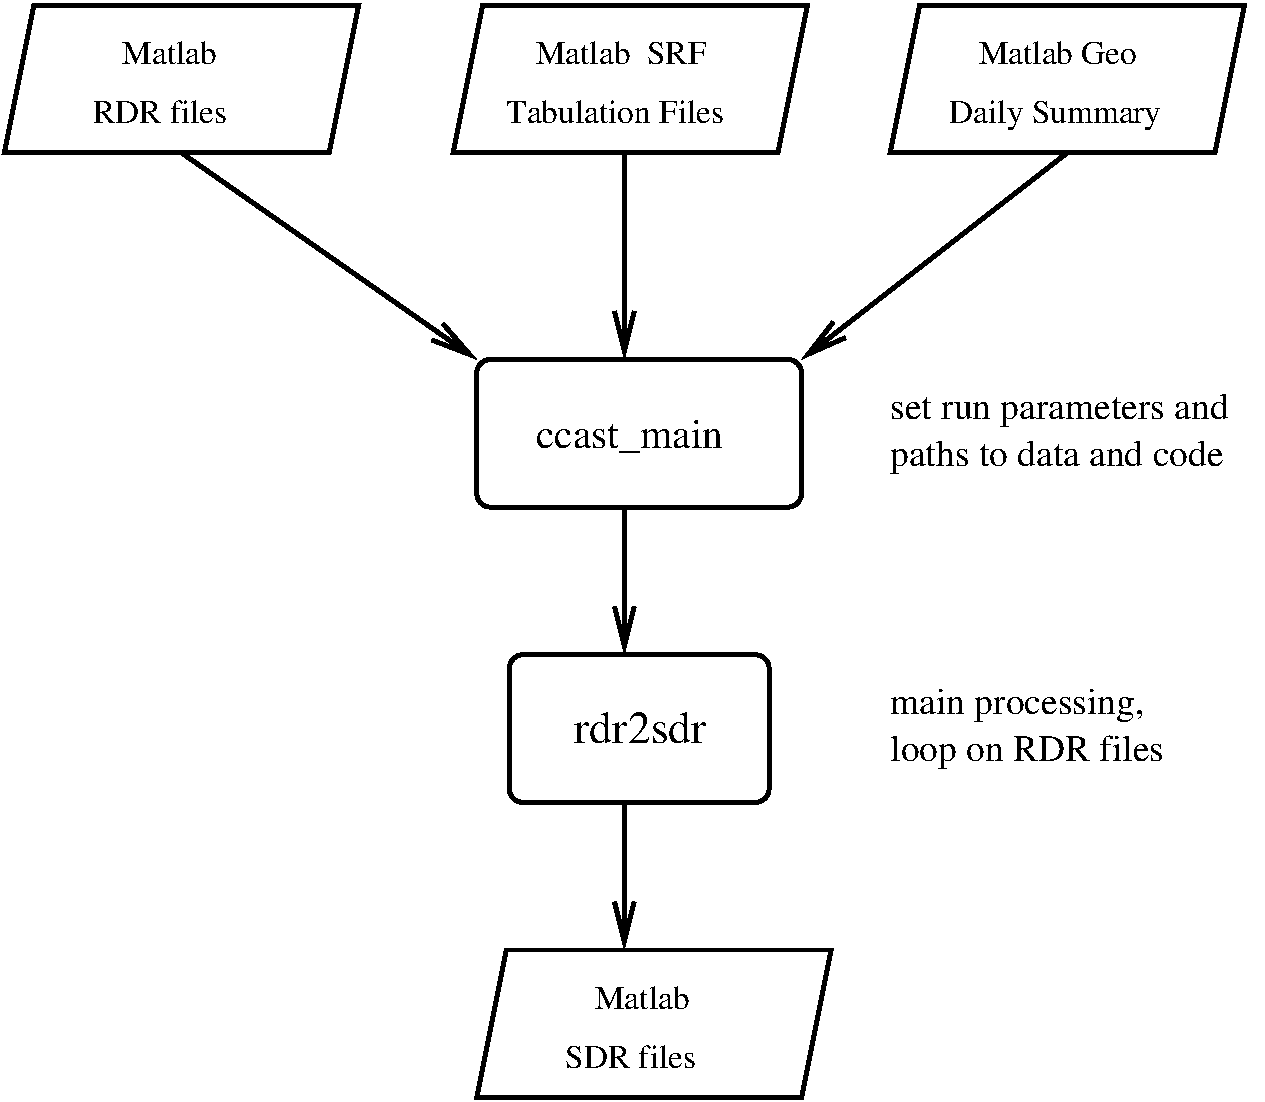
\includegraphics[scale=0.4]{figures/mainpro.pdf}
\end{center}

\end{frame}
%----------- slide --------------------------------------------------%
\begin{frame}
\frametitle{main processing}

ccast\_main sets parameters and paths and calls rdr2sdr, which loops
on Matlab RDR files, typically one set per day.  The main processing
steps in rdr2sdr are

\begin{itemize}
  \item load the Matlab RDR data
  \item process sci and eng support data
  \item order and validate interferogram data
  \item group interferogram data into scans
  \item take interferograms to count spectra
  \item take ICT and space look moving averages
  \item do radiometric and spectral calibration
  \item save the SDR data as HDF5 mat files
\end{itemize}

\end{frame}
%----------- slide --------------------------------------------------%
\begin{frame}
\frametitle{design notes}

\begin{itemize}

  \item control flow is transparent, with almost no control flags
    and no global variables

  \item interferometric and instrument parameters are set in the
    function inst\_params, and runtime parameters in ccast\_main.

  \item data is organized by scans rather than granules.  The output
    SDR files follow the \noaa\ RDR input files but shift the data
    so that the SDR files always start with FOR 1.
   
  \item there is extensive L0 to L1a quality control but currently
    no explicit QC for the final calibrated product beyond keeping
    the complex residual

\end{itemize}

\end{frame}
%----------- slide --------------------------------------------------%
\begin{frame}
\frametitle{performance}

\begin{itemize} 
  \item \ccast\ produces high-quality calibrated radiances and high
    resolution processing has been an option from the start

  \item although it borrows significantly from the \noaa\ ATBD, key
    features such as the ILS, SA interpolation, and the form of the
    calibration equation were developed independently and in many
    cases have been adopted by other groups.

  \item runtime performance is reasonable.  Running as a single
    task, rdr2sdr takes between one and two minutes to processes 
    a 60-scan RDR file

  \item reliability is good.  We have repeatedly reprocessed all
    data from mission start with no problems.

\end{itemize} 

\end{frame}
%----------- slide --------------------------------------------------%
\begin{frame}
\frametitle{getting started}

\begin{itemize} 
   \item to download the ccast repo \\ 
     \hspace{10pt} git clone https://github.com/strow/ccast.git
   \item to update a local copy of the ccast repo \\ 
     \hspace{10pt} git pull origin master
   \item see ccast/README for info on installation and testing, and
     for URLS to test data and sample SRF tabulations
   \item see ccast/doc for
     \begin{itemize}
       \item ccast\_intro.pdf -- this document
       \item ccast\_eqns.pdf -- ILS and main calibration equations
       \item ccast\_sdr.txt -- SDR output data format and fields
       \item finterp.pdf -- notes on Fourier interpolation
     \end{itemize} 
\end{itemize} 

\end{frame}
%----------- slide --------------------------------------------------%
\end{document}
